
\section[{A Gentle Introduction to XML}]{A Gentle Introduction to XML}\label{SG}\par
The encoding scheme defined by these Guidelines is formulated as an application of the Extensible Markup Language (XML) (\cite{XMLREC}). XML is widely used for the definition of device-independent, system-independent methods of storing and processing texts in electronic form. It is now also the interchange and communication format used by many applications on the World Wide Web. In the present chapter we informally introduce some of its basic concepts and attempt to explain to the reader encountering them for the first time how and why they are used in the TEI scheme. More detailed technical accounts of TEI practice in this respect are provided in chapters \textit{\hyperref[USE]{23.\ Using the TEI}}, \textit{\hyperref[ST]{1.\ The TEI Infrastructure}}, and \textit{\hyperref[TD]{22.\ Documentation Elements}} of these Guidelines.\par
Strictly speaking, XML is a \textit{metalanguage}, that is, a language used to describe other languages, in this case, \textit{markup} languages. Historically, the word \textit{markup} has been used to describe annotation or other marks within a text intended to instruct a compositor or typist how a particular passage should be printed or laid out. Examples include wavy underlining to indicate boldface, special symbols for passages to be omitted or printed in a particular font, and so forth. As the formatting and printing of texts was automated, the term was extended to cover all sorts of special codes inserted into electronic texts to govern formatting, printing, or other processing.\par
Generalizing from that sense, we define \textit{markup}, or (synonymously) \textit{encoding}, as any means of making explicit an interpretation of a text. Of course, all printed texts are implicitly encoded (or marked up) in this sense: punctuation marks, capitalization, disposition of letters around the page, even the spaces between words all might be regarded as a kind of markup, the purpose of which is to help the human reader determine where one word ends and another begins, or how to identify gross structural features such as headings or simple syntactic units such as dependent clauses or sentences. Encoding a text for computer processing is, in principle, like transcribing a manuscript from \textit{scriptio continua}\footnote{In the ‘continuous writing’ characteristic of manuscripts from the early classical period, words are written continuously with no intervening spaces or punctuation.}; it is a process of making explicit what is conjectural or implicit, a process of directing the user as to how the content of the text should be (or has been) interpreted.\par
By \textit{markup language} we mean a set of markup conventions used together for encoding texts. A markup language must specify how markup is to be distinguished from text, what markup is allowed, what markup is required, and what the markup means. XML provides the means for doing the first three; documentation such as these Guidelines is required for the last.\par
The present chapter attempts to give an informal introduction to those parts of XML of which a proper understanding is necessary to make best use of these Guidelines. The interested reader should also consult one or more of the many excellent introductory textbooks and web sites now available on the subject.\footnote{New textbooks and websites about XML appear at regular intervals and to select any one of them would be invidious.  some recommended online courses include \url{http://www.w3schools.com/xml/default.asp} and \url{https://www.ibm.com/developerworks/xml/tutorials/xmlintro/xmlintro.html}.}
\subsection[{What's Special about XML?}]{What's Special about XML?}\label{SG11}\par
XML has three highly distinctive advantages: \begin{enumerate}
\item it places emphasis on descriptive rather than procedural markup;
\item it distinguishes the concepts of syntactic correctness and of \textit{validity} with respect to a \textit{document type definition};
\item it is independent of any one hardware or software system.
\end{enumerate} These three aspects are discussed briefly below, and then in more depth in the remainder of this chapter.\par
XML is frequently compared with HTML, the language in which web pages have generally been written, which shares some of the above characteristics. Compared with HTML, however, XML has some other important features: \begin{itemize}
\item XML is {\itshape extensible}: it does not consist of a fixed set of tags;
\item XML documents must be {\itshape well-formed} according to a defined syntax;
\item an XML document can be formally {\itshape validated} against a set of schema rules for consistent application;
\item XML is more interested in the meaning of data than in its presentation.
\end{itemize} 
\subsubsection[{Descriptive Markup}]{Descriptive Markup}\label{SG111}\par
In a descriptive markup system, the markup codes used do little more than categorize parts of a document. Markup codes such as <para> or \texttt{\textbackslash end\{list\}} simply identify a portion of a document and assert of it that ‘the following item is a paragraph’, or ‘this is the end of the most recently begun list’, etc. By contrast, a procedural markup system defines what processing is to be carried out at particular points in a document: ‘call procedure PARA with parameters 42, b, and x here’ or ‘move the left margin 2 quads left, move the right margin 2 quads right, skip down one line, and go to the new left margin,’ etc. In XML, the instructions needed to process a document for some particular purpose (for example, to format it) are sharply distinguished from the markup used to describe it.\par
Usually, the markup or other information needed to process a document will be maintained separately from the document itself, typically in a distinct document called a \textit{stylesheet}, though it may do much more than simply define the rendition or visual appearance of a document.\footnote{We do not here discuss in any detail the ways that a stylesheet can be used or defined, nor do we discuss the popular W3C Stylesheet Languages XSLT and CSS. See further \cite{XSL11}, \cite{XSLT}, and \cite{CSS1}.}\par
When descriptive markup is used, the same document can readily be processed in many different ways, using only those parts of it which are considered relevant. For example, a content analysis program might disregard entirely the footnotes embedded in an annotated text, while a formatting program might extract and collect them all together for printing at the end of each chapter. Different kinds of processing can be carried out with the same part of a file. For example, one program might extract names of persons and places from a document to create an index or database, while another, operating on the same text, but using a different stylesheet, might print names of persons and places in a distinctive typeface.
\subsubsection[{Types of Document}]{Types of Document}\label{SG112}\par
A second key aspect of XML is its notion of a \textit{document type}: documents are regarded as having types, just as other objects processed by computers do. The type of a document is formally defined by its constituent parts and their structure. The definition of a ‘report’, for example, might be that it consisted of a ‘title’ and possibly an ‘author’, followed by an ‘abstract’ and a sequence of one or more ‘paragraphs’. Anything lacking a title, according to this formal definition, would not formally be a report, and neither would a sequence of paragraphs followed by an abstract, whatever other report-like characteristics these might have for the human reader.\par
If documents are of known types, a special-purpose program (called a \textit{parser}), once provided with an unambiguous definition of a document type, can check that any document claiming to be of that type does in fact conform to the specification. A parser can check that all elements specified for a particular document type are present and no others, that they are combined in appropriate ways, correctly ordered, and so forth. More significantly, different documents of the same type can be processed in a uniform way. Programs can be written which take advantage of the knowledge encapsulated in the document type information, and which can thus behave in a more ‘intelligent’ fashion.
\subsubsection[{Data Independence}]{Data Independence}\label{SG113}\par
A basic design goal of XML is to ensure that documents encoded according to its provisions can move from one hardware and software environment to another without loss of information. The two features discussed so far both address this requirement at an abstract level; the third feature addresses it at the level of the strings of data characters that make up a document. All XML documents, whatever languages or writing systems they employ, use the same underlying character encoding (that is, the same method of representing as binary data those graphic forms making up a particular writing system).\footnote{See \textit{Extensible Markup Language (XML) 1.0}, available from \url{http://www.w3.org/TR/REC-xml/}, Section 2.2 Characters.} This encoding is defined by an international standard,\footnote{ISO/IEC 10646-1993 \textit{Information Technology — Universal Multiple-Octet Coded Character Set} (UCS)} which is implemented by a universal character set maintained by an industry group called the Unicode Consortium, and known as Unicode.\footnote{See \url{http://www.unicode.org/}} Unicode provides a standardized way of representing any of the many thousands of discrete symbols making up the world's writing systems, past and present.\par
Most modern computing systems now support Unicode directly; for those which do not, XML provides a mechanism for the indirect representation of single characters by means of their character number, known as \textit{character references}; see further \textit{\hyperref[SG-er]{v.7.1\ Character References}}.
\subsection[{Textual Structures}]{Textual Structures}\label{SG12}\par
A text is not an undifferentiated sequence of words, much less of bytes. For different purposes, it may be divided into many different units, of different types or sizes. A prose text such as this one might be divided into sections, chapters, paragraphs, and sentences. A verse text might be divided into cantos, stanzas, and lines. Once printed, sequences of prose and verse might be divided into volumes, gatherings, and pages.\par
Structural units of this kind are most often used to identify specific locations or refer to points within a text (‘the third sentence of the second paragraph in chapter ten’; ‘canto 10, line 1234’; ‘page 412’, etc.) but they may also be used to subdivide a text into meaningful fragments for analytic purposes (‘is the average sentence length of section 2 different from that of section 5?’ ‘how many paragraphs separate each occurrence of the word \textit{nature}? how many pages?’). Other structural units are more clearly analytic, in that they characterize a section of a text. A dramatic text might regard each speech by a different character as a unit of one kind, and stage directions or pieces of action as units of another kind. Such an analysis is less useful for locating parts of the text (‘the 93rd speech by Horatio in Act 2’) than for facilitating comparisons between the words used by one character and those of another, or those used by the same character at different points of the play.\par
In a prose text one might similarly wish to regard as units of different types passages in direct or indirect speech, passages employing different stylistic registers (narrative, polemic, commentary, argument, etc.), passages of different authorship and so forth. And for certain types of analysis (most notably textual criticism) the physical appearance of one particular printed or manuscript source may be of importance: paradoxically, one may wish to use descriptive markup to describe presentational features such as typeface, line breaks, use of whitespace and so forth.\par
These textual structures overlap with one another in complex and unpredictable ways. Particularly when dealing with texts as instantiated by paper technology, the reader needs to be aware of both the physical organization of the book and the logical structure of the work it contains. Many great works (Sterne's \textit{Tristram Shandy} for example) cannot be fully appreciated without an awareness of the interplay between narrative units (such as chapters or paragraphs) and presentational ones (such as page divisions). For many types of research, the interplay among different levels of analysis is crucial: the extent to which syntactic structure and narrative structure mesh, or fail to mesh, for example, or the extent to which phonological structures reflect morphology.
\subsection[{XML Structures}]{XML Structures}\label{SG13}\par
This section describes the simple and consistent mechanism for the markup or identification of textual structure provided by XML. It also describes the methods XML provides for the expression of rules defining how units of textual structure can meaningfully be combined in a text.
\subsubsection[{Elements}]{Elements}\label{SG131}\par
The technical term used in XML for a textual unit, viewed as a structural component, is \textit{element}. Different types of elements are given different names, but XML provides no way of expressing the meaning of a particular type of element, other than its relationship to other element types. That is, all one can say about an element called (say) \texttt{<blort>} is that instances of it may (or may not) occur within elements of type \texttt{<farble>}, and that it may (or may not) be decomposed into elements of type \texttt{<blortette>}. It should be stressed that XML is entirely unconcerned with the \textit{semantics} of textual elements, because these are considered to be application dependent. It is up to the creators of XML vocabularies (such as these Guidelines) to choose intelligible element names and to define their intended use in text markup. That is the chief purpose of documents such as the TEI Guidelines. From the need to choose element names indicative of function comes the technical term for the name of an element type, which is \textit{generic identifier}, or GI.\par
Within a marked-up text (a \textit{document instance}), each element must be explicitly marked or tagged in some way. This is done by inserting a tag at the beginning of the element (a \textit{start-tag}) and another at its end (an \textit{end-tag}). The start- and end-tag pair are used to bracket off element occurrences within the running text, in rather the same way as different types of parentheses or quotation marks are used in conventional punctuation. For example, a quotation element in a text might be tagged as follows: \par\bgroup\index{quote=<quote>|exampleindex}\exampleFont \begin{shaded}\noindent\mbox{}... Rosalind's\mbox{}\newline 
 remarks {<\textbf{quote}>}This is the silliest stuff that ere I heard\mbox{}\newline 
 of!{</\textbf{quote}>} clearly indicate ...\end{shaded}\egroup\par \noindent  As this example shows, a start-tag takes the form <quote>, where the opening angle bracket indicates the start of the start-tag, ‘quote’ is the generic identifier of the element that is being delimited, and the closing angle bracket indicates the end of the start-tag. An end-tag takes an identical form, except that the opening angle bracket is followed by a solidus (slash) character, so that the corresponding end-tag is </quote>.\footnote{Because the opening angle bracket has this special function in an XML document, special steps must be taken to use that character for other purposes (for example, as the mathematical less-than operator); see further section \textit{\hyperref[SG-er]{v.7.1\ Character References}}.} The material between the start-tag and the end-tag (the string of words ‘This is the silliest stuff that ere I heard of’ in the example above) is known as the \textit{content} of the element. Sometimes there may be nothing between the start and the end-tag; in this case the two may optionally be merged together into a single composite tag with the solidus at the end, like this: <quote/>.
\subsubsection[{Content Models: an Example}]{Content Models: an Example}\label{SG132}\par
An element may be \textit{empty}, that is, it may have no content at all, or it may contain just a sequence of characters with no other elements. Often, however, elements of one type will be \textit{embedded} (contained entirely) within elements of a different type.\par
To illustrate this, we will consider a very simple structural model. Let us assume that we wish to identify within an anthology only poems, their headings, and the stanzas and lines of which they are composed. In XML terms, our \textit{document type} is the \textit{anthology}, and it consists of a series of \textit{poem}s. Each poem has embedded within it one element, a \textit{heading}, and several occurrences of another, a \textit{stanza}, each stanza having embedded within it a number of \textit{line} elements. Fully marked up, a text conforming to this model might appear as follows: \par\bgroup\exampleFont \begin{shaded}\noindent\mbox{}{<\textbf{anthology}>}\mbox{}\newline 
\hspace*{1em}{<\textbf{poem}>}\mbox{}\newline 
\hspace*{1em}\hspace*{1em}{<\textbf{heading}>}The SICK ROSE{</\textbf{heading}>}\mbox{}\newline 
\hspace*{1em}\hspace*{1em}{<\textbf{stanza}>}\mbox{}\newline 
\hspace*{1em}\hspace*{1em}\hspace*{1em}{<\textbf{line}>}O Rose thou art sick.{</\textbf{line}>}\mbox{}\newline 
\hspace*{1em}\hspace*{1em}\hspace*{1em}{<\textbf{line}>}The invisible worm,{</\textbf{line}>}\mbox{}\newline 
\hspace*{1em}\hspace*{1em}\hspace*{1em}{<\textbf{line}>}That flies in the night{</\textbf{line}>}\mbox{}\newline 
\hspace*{1em}\hspace*{1em}\hspace*{1em}{<\textbf{line}>}In the howling storm:{</\textbf{line}>}\mbox{}\newline 
\hspace*{1em}\hspace*{1em}{</\textbf{stanza}>}\mbox{}\newline 
\hspace*{1em}\hspace*{1em}{<\textbf{stanza}>}\mbox{}\newline 
\hspace*{1em}\hspace*{1em}\hspace*{1em}{<\textbf{line}>}Has found out thy bed{</\textbf{line}>}\mbox{}\newline 
\hspace*{1em}\hspace*{1em}\hspace*{1em}{<\textbf{line}>}Of crimson joy:{</\textbf{line}>}\mbox{}\newline 
\hspace*{1em}\hspace*{1em}\hspace*{1em}{<\textbf{line}>}And his dark secret love{</\textbf{line}>}\mbox{}\newline 
\hspace*{1em}\hspace*{1em}\hspace*{1em}{<\textbf{line}>}Does thy life destroy.{</\textbf{line}>}\mbox{}\newline 
\hspace*{1em}\hspace*{1em}{</\textbf{stanza}>}\mbox{}\newline 
\hspace*{1em}{</\textbf{poem}>}\mbox{}\newline 
\textit{<!-- more poems go here -->}\mbox{}\newline 
{</\textbf{anthology}>}\end{shaded}\egroup\par \par
It should be stressed that this example does \textit{not} use the names proposed for corresponding elements elsewhere in these Guidelines: the above is thus \textit{not} a valid TEI document.\footnote{The element names here have been chosen for clarity of exposition; there is, however, a TEI element corresponding to each.} It will, however, serve as an introduction to the basic notions of XML. Whitespace and line breaks have been added to the example for the sake of visual clarity only; they have no particular significance in the XML encoding itself. Also, the line \par\hfill\bgroup\exampleFont\vskip 10pt\begin{shaded}
\obeyspaces <!-- more poems go here -->\end{shaded}
\par\egroup 
 is an XML \textit{comment} and is not treated as part of the text.\par
As it stands, the above example is what is known as a \textit{well-formed} XML document because it obeys the following simple rules: \begin{enumerate}
\item there is a single element enclosing the whole document: this is known as the \textit{root element} (\texttt{<anthology>} in our case);
\item each element is completely contained by the root element, or by an element that is so contained; elements do not partially overlap one another;
\item a tag explicitly marks the start and end of each element.
\end{enumerate}\par
A well-formed XML document can be processed in a number of useful ways. A simple indexing program could extract only the relevant text elements in order to make a list of headings, first lines, or words used in the poem text; a simple formatting program could insert blank lines between stanzas, perhaps indenting the first line of each, or inserting a stanza number. Different parts of each poem could be typeset in different ways. A more ambitious analytic program could relate the use of punctuation marks to stanzaic and metrical divisions.\footnote{Note that this simple example has not addressed the problem of marking elements such as sentences explicitly; the implications of this are discussed in section \textit{\hyperref[SG152]{v.5\ Complicating the Issue}}.} Scholars wishing to see the implications of changing the stanza or line divisions chosen by the editor of this poem can do so simply by altering the position of the tags. And of course, the text as presented above can be transported from one computer to another and processed by any program (or person) capable of making sense of the tags embedded within it with no need for the sort of transformations and translations needed for files which have been saved in one or other of the proprietary formats preferred by most word-processing programs.\par
As we noted above, one of the attractions of XML is that it enables us to apply our own names for the elements rather than requiring us always to use names predefined by other agencies. Clearly, however, if we wish to exchange our poems with others, or to include poems others have marked up in our anthology, we will need to know a bit more about the names used for the tags. The means that XML provides for this is called a \textit{namespace}. In our simple example, the tags just contain a simple name. As we shall see, it is also possible to use tags that include a \textit{qualified name}, that is, a name with an optional prefix identifying the set of names to which it belongs. For example, we have defined an element \texttt{<line>} for the purpose of marking lines of verse. Another person might, however, define an element called \texttt{<line>} for the purpose of marking typographic lines, or drawn lines. Because of these different meanings, if we wish to share data it will be necessary to distinguish the two ‘line’ components in our marked-up texts. This is achieved by including a \textit{namespace prefix} within the markup, for example like this: \par\hfill\bgroup\exampleFont\vskip 10pt\begin{shaded}
\obeyspaces  <my:line>This is one of my lines</my:line> \newline
<!-- ... --> \newline
<yr:line>This is one of your lines</yr:line>\end{shaded}
\par\egroup 
 This feature is particularly important if we have different definitions of what a ‘line’ is, of course, but there are many occasions when it is useful to distinguish groups of tags belonging to different ‘markup vocabularies’; we discuss this further below (\textit{\hyperref[SGname]{v.7.2\ Namespaces}}). One particularly useful namespace prefix is predefined for XML: it is \texttt{xml} and we will see examples of its use below.\par
Namespaces allow us to represent the fact that a name belongs to a group of names, but don't allow us to do much more by way of checking the integrity or accuracy of our tagging. Simple well-formedness alone is not enough for the full range of what might be useful in marking up a document. It might well be useful if, in the process of preparing our digital anthology, a computer system could check some basic rules about how stanzas, lines, and headings can sensibly co-occur in a document. It would be even more useful if the system could check that stanzas are always tagged <stanza> and not occasionally <canto> or <Stanza>. An XML document in which such rules have been checked is technically known as a \textit{valid} document, and the ability to perform such validation is one of the key advantages of using XML. To carry this out, some way of formally stating the criteria for successful validation is necessary: in XML this formal statement is provided by an additional document known as a \textit{schema}.\footnote{The older terms \textit{Document Type Declaration} and \textit{Document Type Definition}, both abbreviated as DTD, may also be encountered. Throughout these Guidelines we use the term \textit{schema} for any kind of formal document grammar.}
\subsection[{Validating a Document's Structure}]{Validating a Document's Structure}\label{SG14}\par
The design of a schema may be as lax or as restrictive as the occasion warrants. A balance must be struck between the convenience of following simple rules and the complexity of handling real texts. This is particularly the case when the rules being defined relate to texts that already exist: the designer may have only the haziest of notions as to an ancient text's original purpose or meaning and hence find it very difficult to specify consistent rules about its structure. On the other hand, where a new text is being prepared to an exact specification, for entry into a textual database of some kind for example, the more precisely stated the rules, the better they can be enforced. Even in marking up an existing text, a restrictive set of schema rules may be beneficial, especially when applied to test a particular view or hypothesis about the text. A schema designed for use by a small project or team is likely to take a different position on such issues than one intended for use by a large and possibly fragmented community. It is important to remember that every schema results from an interpretation of a text. There is no single schema encompassing the absolute truth about any text, although it may be convenient to privilege some schemas above others for particular types of analysis.\par
XML is widely used in environments where uniformity of document structure is a major desideratum. In the production of technical documentation, for example, it is of major importance that sections and subsections should be properly nested, that cross-references should be properly resolved and so forth. In such situations, documents are seen as raw material to match against predefined sets of rules. As discussed above, however, the use of simple rules can also greatly simplify the task of tagging accurately elements of less rigidly constrained texts. By making these schema rules explicit, scholars reduce their own burdens with consistently marking up and verifying the electronic text. By defining and sharing their schema rules, scholars openly express a project-specific interpretation of the structure and significant particularities of the text being encoded.\par
Schema validation for XML is usually written in the RELAX NG language (\url{http://relaxng.org/}) originally developed within the OASIS Technical Committee and now an ISO standard\footnote{\xref{https://www.iso.org/standard/52348.html}{ISO/IEC FDIS 19757-2 Document Schema Definition Language (DSDL) -- Part 2: Regular-grammar-based validation -- RELAX NG}}, though other older methods include the Document Type Definition (DTD) language which XML inherited from SGML and the XML Schema language (\url{http://www.w3.org/XML/Schema}) defined by the W3C.\footnote{Schema validation languages co-evolved with early markup language specifications, as summarized in \xref{http://xml.coverpages.org/Jelliffe-schema-family-tree3-20061130.jpg}{Rick Jelliffe's Family Tree of Schema Languages for Markup Languages}.} In this chapter, and throughout these Guidelines, we give examples using the ‘compact syntax’ of RELAX NG for ease of reading. The specifications for the TEI Guidelines are first expressed in the TEI language itself and a RELAX NG schema is generated from them for processing convenience. Details about schema customization using the TEI ODD language are addressed in \textit{\hyperref[TD]{22.\ Documentation Elements}}, \textit{\hyperref[MD]{23.3.\ Customization}} and \textit{\hyperref[IM]{23.5.\ Implementation of an ODD System}}.
\subsubsection[{An Example Schema}]{An Example Schema}\label{SG141bis}\par
For the purposes of illustrating how a schema works to restrict how XML may be written, we use the RELAX NG compact syntax in what follows. The following schema can be used to validate our example poem: \par\hfill\bgroup\exampleFont\vskip 10pt\begin{shaded}
\obeyspaces anthology\textunderscore p = element anthology ❴ poem\textunderscore p+ ❵\newline
poem\textunderscore p = element poem ❴ heading\textunderscore p?, stanza\textunderscore p+ ❵\newline
stanza\textunderscore p = element stanza ❴line\textunderscore p+❵\newline
heading\textunderscore p = element heading ❴ text ❵\newline
line\textunderscore p = element line ❴ text ❵\newline
start = anthology\textunderscore p\end{shaded}
\par\egroup 
\par
Note that this is not the only way in which a RELAX NG schema might be written; we have adopted this idiom, however, because it matches that used throughout the rest of these Guidelines.\par
A RELAX NG schema expresses rules about the possible structure of a document in terms of \textit{patterns}; that is, it defines a number of named patterns, each of which acts as a kind of template against which an input document can be matched. The meaning of a pattern is expressed in a schema either by reference to other patterns, or to a small number of fundamental built-in concepts, as we shall see. In the example above, the word to the left of the equals sign is the pattern's name, and the material following it declares a meaning for the pattern. Patterns may also be of particular types; the ones that interest us here are called \textit{element patterns} and \textit{attribute patterns}. In this example we see definitions for five element patterns. Note that we have used similar names for the pattern and the element which the pattern describes: so, for example, the line \texttt{anthology\textunderscore p = element anthology \{poem\textunderscore p+\}} defines an element pattern called \texttt{anthology\textunderscore p}, the value of which defines an element called \texttt{anthology}. These naming conventions are arbitrary; we could use the same name for the pattern as for the element, but we want to make clear that the two are syntactically quite distinct. The name, or \textit{generic identifier}, of the element follows the word ‘element’, and the \textit{content model} for the element is given within the curly braces following that. Each of these parts is discussed further below.\par
The last line of the schema above tells a RELAX NG validator which element (or elements) in a document can be used as the root element: in our case only \texttt{<anthology>}. This enables the validator to detect whether a particular document is well-formed but incomplete; it also simplifies the processing task by providing an ‘entry point’.
\paragraph[{Generic Identifier}]{Generic Identifier}\label{SG141x}\par
Following the word ‘element’ each pattern declaration gives the generic identifier (often abbreviated to GI) of the element being defined, for example \textit{poem}, \textit{heading}, etc. A GI may contain letters, digits, hyphens, underscore characters, or full stops, but must begin with a letter and may not contain a space.\footnote{In XML, a single colon may also appear in a GI, where it has a special significance related to the use of \textit{namespaces}, as further discussed in section \textit{\hyperref[SGname]{v.7.2\ Namespaces}}. The characters defined by Unicode as \textit{combining characters} and as \textit{extenders} are also permitted, as are logograms such as Chinese characters.} Uppercase and lowercase letters are quite distinct: an element with the GI \texttt{<foo>} is \textit{not} the same as an element with the GI \texttt{<Foo>}; the root element of a TEI-conformant document is \hyperref[TEI.TEI]{<TEI>}, \textit{not} \texttt{<tei>}.
\paragraph[{Content Model}]{Content Model}\label{SG143}\par
The second part of each declaration, enclosed in curly braces, is called the \textit{content model} of the element being defined, because it specifies what may legitimately be contained within it. In RELAX NG, the content model is defined in terms of other patterns, either by embedding them, or (as in our examples above) by naming or referring to them. The RELAX NG compact syntax also uses a small number of reserved words to identify other possible contents for an element, of which by far the most commonly encountered is \texttt{text}, as in this example: it means that the element being defined may contain any valid character data, but no elements. If an XML document is thought of as a structure like a family tree, with a single ancestor at the top (in our case, this would be <anthology>), then almost always, following the branches of the tree downwards (for example, from \texttt{<anthology>} to \texttt{<poem>} to \texttt{<stanza>} to \texttt{<line>} and \texttt{<heading>}) will lead eventually to \texttt{text}. In our example, \texttt{<heading>} and \texttt{<line>} are so defined, since their content models say \texttt{text} only and name no embedded elements.
\paragraph[{Occurrence Indicators}]{Occurrence Indicators}\label{SG144}\par
The declaration for \texttt{<stanza>} in the example above states that a stanza consists of one or more lines. It uses an \textit{occurrence indicator} (the plus sign) to indicate how many times something matching the pattern \texttt{line\textunderscore p} may be repeated. There are three occurrence indicators: the plus sign, the question mark, and the asterisk or star. The plus sign means that the pattern can match one or more times; the question mark means that it may match at most once but is not mandatory; the star means that the pattern concerned is not mandatory, but may match more than once. Thus, if the content model for \texttt{<stanza>} were \texttt{\{line\textunderscore p*\}}, stanzas with no lines would be possible as well as those with more than one line. If it were \texttt{\{line\textunderscore p?\}}, again empty stanzas would be permitted, but no stanza could have more than a single line. The declaration for \texttt{<poem>} in the example above thus states that a \texttt{<poem>} cannot have more than one heading, but may have none, and that it must have at least one \texttt{<stanza>} and may have several.
\paragraph[{Connectors}]{Connectors}\label{SG145}\par
The content model \texttt{\{heading\textunderscore p?, stanza\textunderscore p+\}} contains more than one component, and thus needs additionally to specify the order in which these patterns (\texttt{<heading\textunderscore p>} and \texttt{<stanza\textunderscore p>}) may appear. This ordering is determined by the \textit{connector} (the comma) used between its components. The comma connector indicates that the patterns concerned must appear in the sequence given. Another commonly encountered connector is the vertical bar, representing alternation. If the comma in this example were replaced by a vertical bar, then a \texttt{<poem>} would consist of either a heading or just stanzas—but not both!
\paragraph[{Groups}]{Groups}\label{SG146}\par
In our example so far, the components of each content model have been either single patterns or \texttt{text}. We often need to define content models in more complicated ways, in which the components are lists of patterns, combined by connectors. Such lists may also be modified by occurrence indicators and themselves combined by connectors. To demonstrate these facilities, let us expand our example so that it may include non-stanzaic types of verse. For the sake of demonstration, we will categorize poems as one of the following: \textit{stanzaic}, \textit{couplets}, or \textit{blank} (or \textit{stichic}). A blank-verse poem consists simply of lines (we ignore the possibility of verse paragraphs for the moment),  so no additional elements need be defined for it. We could define a couplet as a \texttt{<firstLine>} followed by a \texttt{<secondLine>}, which distinction might be useful in a study of rhyme schemes.\footnote{This example is probably not a good practice for most XML projects, since XPath provides ways of distinguishing elements in an XML structure by their position, or the order in which they appear in relation to one another, without the need to give them distinct names.} \par\hfill\bgroup\exampleFont\vskip 10pt\begin{shaded}
\obeyspaces couplet\textunderscore p = element couplet ❴firstLine\textunderscore p, secondLine\textunderscore p❵\end{shaded}
\par\egroup 
   \par
The patterns firstLine\textunderscore p and secondLine\textunderscore p define elements \texttt{<firstLine>} and \texttt{<secondLine>}; these will have exactly the same content model as the existing \texttt{<line>} element. We will therefore add the following two lines to our example schema: \par\hfill\bgroup\exampleFont\vskip 10pt\begin{shaded}
\obeyspaces firstLine\textunderscore p = element firstLine ❴text❵ secondLine\textunderscore p = element secondLine ❴text❵\end{shaded}
\par\egroup 
 Next, we can change the declaration for the \texttt{<poem>} element to include all three possibilities: \par\hfill\bgroup\exampleFont\vskip 10pt\begin{shaded}
\obeyspaces  poem\textunderscore p = element poem\newline
❴ heading\textunderscore p?, (stanza\textunderscore p+ | couplet\textunderscore p+ | line\textunderscore p+) ❵\end{shaded}
\par\egroup 
 That is, a poem consists of an optional heading, followed by one or several stanzas, or one or several couplets, or one or several lines. Note the difference between this declaration and the following: \par\hfill\bgroup\exampleFont\vskip 10pt\begin{shaded}
\obeyspaces poem\textunderscore p = element poem\newline
❴heading\textunderscore p?, (stanza\textunderscore p | couplet\textunderscore p | line\textunderscore p)+ ❵\end{shaded}
\par\egroup 
 The second version, by applying the occurrence indicator to the group rather than to each element within it, would allow a single poem to contain a mixture of stanzas, couplets, and lines.\par
A group of this kind can contain \texttt{text} as well as named elements: this combination, known as \textit{mixed content}, allows for elements in which the sub-components appear with intervening stretches of character data. For example, if we wished to mark place names wherever they appear inside our verse lines, then, assuming we have also added a pattern for the \texttt{<name>} element, we could change the definition for \texttt{<line>} to \par\hfill\bgroup\exampleFont\vskip 10pt\begin{shaded}
\obeyspaces line\textunderscore p = element\newline
line ❴ (text | name\textunderscore p )* ❵\end{shaded}
\par\egroup 
\par
Some XML schema languages place no constraints on the way that mixed content models may be defined, but in the XML DTD language, when \texttt{text} appears with other elements in a content model, it must always appear as the first option in an alternation; it may appear once only, and in the outermost model group; and if the group containing it is repeated, the star operator must be used. Although these constraints are not strictly necessary in RELAX NG schemas, all TEI content models currently obey them.\par
Quite complex models can be built in this way, to match the structural complexity of many types of text. For example, consider the case of stanzaic verse in which a refrain or chorus appears. Like a stanza, a refrain consists of repetitions of the line element. A refrain can appear at the start of a poem only, or as an optional addition following each stanza. This could be expressed by a pattern such as the following: \par\hfill\bgroup\exampleFont\vskip 10pt\begin{shaded}
\obeyspaces refrain\textunderscore p = element refrain ❴line\textunderscore p+❵\newline
poem\textunderscore p = element poem   ❴heading\textunderscore p?, ( line\textunderscore p+ | (refrain\textunderscore p?, (stanza\textunderscore p,\newline
refrain\textunderscore p?)+ )) ❵\end{shaded}
\par\egroup 
 That is, a poem consists of an optional heading, followed by either a sequence of lines or an unnamed group, which starts with an optional refrain and is followed by one or more occurrences of another group, each member of which is composed of a stanza followed by an optional refrain. A sequence such as \textit{refrain - stanza - stanza - refrain} follows this pattern, as does the sequence \textit{stanza - refrain - stanza - refrain}. The sequence \textit{refrain - refrain - stanza - stanza} does not, however, and neither does the sequence \textit{stanza - refrain - refrain - stanza.} Among other conditions made explicit by this content model are the requirements that at least one stanza must appear in a poem, if it is not composed simply of lines, and that if there is both a heading and a stanza they must appear in that order.\par
Note that the apparent complexity of this model derives from the constraints expressed informally above. A simpler model, such as \par\hfill\bgroup\exampleFont\vskip 10pt\begin{shaded}
\obeyspaces poem\textunderscore p =\newline
element poem ❴heading\textunderscore p?, (line\textunderscore p | refrain\textunderscore p | stanza\textunderscore p)+ ❵\end{shaded}
\par\egroup 
 would not enforce any of them, and would therefore permit such anomalies as a poem consisting only of refrains, or an arbitrary mixture of lines and refrains.\par
It is beyond the scope of this "Gentle Introduction to XML" to provide a complete orientation to schema writing with Relax NG, but interested readers may wish to consult more thorough tutorials on the subject.\footnote{For a complete tutorial introduction to RELAX NG, see \cite{SG-BIBL-1}.} The examples and explanation provided here may be helpful to consult when reading the schema declarations posted for groupings of TEI elements that share the same content model, such as \xref{ref-macro.phraseSeq.html}{macro.phraseSeq}, whose declaration features an example of mixed text and element content. Due to the complexity of the TEI schema as expressed in Relax NG, it is best to customize its content model in TEI itself by writing an ODD, as discussed in \textit{\hyperref[IM]{23.5.\ Implementation of an ODD System}}.
\subsection[{Complicating the Issue}]{Complicating the Issue}\label{SG152}\par
In the simple cases described so far, we have assumed that one can identify the immediate constituents of every element in a textual structure. A poem consists of stanzas, and an anthology consists of poems. Stanzas do not float around unattached to poems or combined into some other unrelated element; a poem cannot contain an anthology. All the elements of a given document type may be arranged into a hierarchic structure like a family tree, with a single ancestor at one end and many children (mostly the elements containing simple text) at the other. For example, we could represent an anthology containing two poems, the first of which contains two four-line stanzas and the second a single stanza, by a tree structure like the following figure:\begin{figure}[htbp]
\noindent\noindent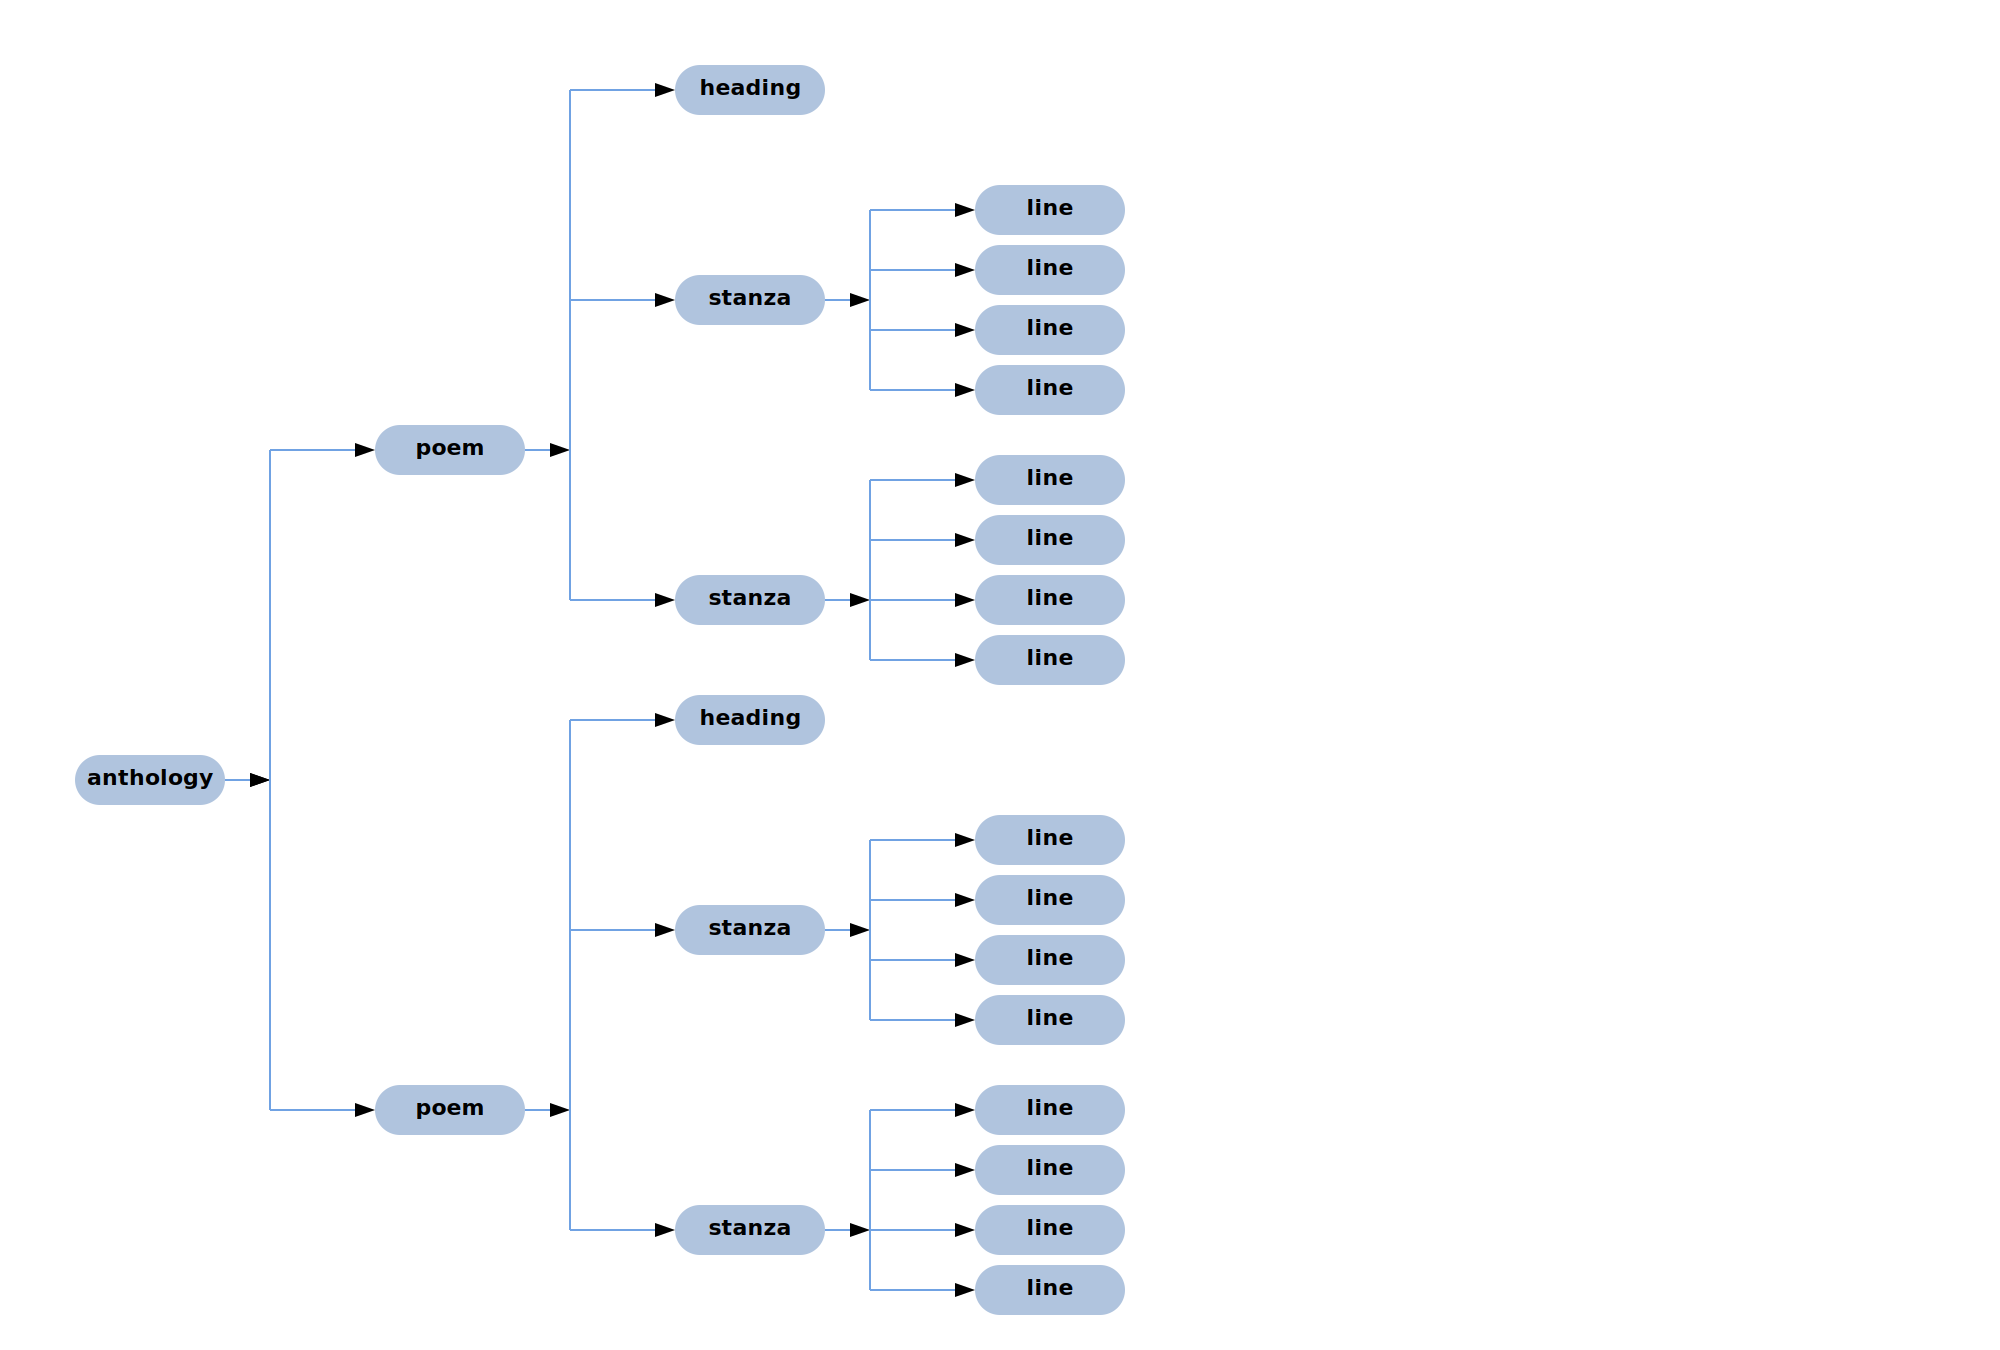
\includegraphics[width=0.8\textwidth,]{Images/xmlFlowChart.png}\end{figure}
\par
This graphic represents the hierarchical structure of an XML document, resembling a family tree. Most XML processing systems now use a standardized way of accessing parts of an XML document called \textit{XPath}.\footnote{The official specification is at \cite{XPATH}; many introductory tutorials are available in the XML references cited above and elsewhere on the Web: good beginners' tutorials include \url{http://dh.obdurodon.org/introduction-xpath.xhtml}, \url{http://www.w3schools.com/xml/xpath\textunderscore intro.asp} and \url{http://www.zvon.org/xxl/XPathTutorial/}, the latter being available in several languages.} XPath gives us a non-graphical way of referring to any part of an XML document: for example, we might refer to the last line of Blake's poem as \texttt{/anthology/poem[1]/stanza[2]/line[4]}. The square brackets here indicate a numerical selection: we are talking about the fourth line in the second stanza of the first poem in the anthology. If we left out all the square-bracketted selections, the corresponding XPath expression would refer to all lines contained by stanzas contained by poems contained by anthologies. An XPath expression can refer to any collection of elements: for example, the expression \texttt{/anthology/poem} refers to all poems in an anthology and the expression \texttt{/anthology/poem/heading} refers to all their headings.\par
The forward slash (‘/’, U+002F SOLIDUS) within an XPath expression behaves in much the same way as a forward slash or backslash does in a filename specification. To use a family tree analogy, a single slash indicates that the item to the immediate left is a parent of the item(s) to the right of it. For example, in the XPath expression \texttt{/anthology/poem}, the single slash between anthology and poem indicates that anthology is a parent of the poem children elements. (The first forward slash in the XPath expression indicates the document node.) In XPath, it is also possible to refer to children, grandchildren, and other descendants of the family tree using two forward slashes together. For example, the XPath expression \texttt{/anthology/poem//line} will refer to all of the lines of all of the stanzas of all the poems, without having to represent the stanza element in the XPath.\par
Clearly, there are many such trees that might be drawn to describe the structure of this or other anthologies. Some of them might be representable as further subdivisions of this tree: for example, we might subdivide the lines into individual words, since in our simple example no word crosses a line boundary. Surprisingly perhaps, this grossly simplified view of what text is (memorably termed an \textit{ordered hierarchy of content objects} (OHCO) view of text by Renear \textit{et al.}\footnote{See \cite{SG-BIBL-2}.}) turns out to be very effective for a large number of purposes. It is not, however, adequate for the full complexity of real textual structures, for which more complex mechanisms need to be employed. There are many other trees that might be drawn which do \textit{not} fit within the anthology model which we have presented so far. We might, for example, be interested in syntactic structures or other linguistic constructs, which rarely respect the formal boundaries of verse. Or, to take a simpler example, we might want to represent the pagination of different editions of the same text.\par
In the OHCO model of text, representation of cases where different elements overlap so that several different trees may be identified in the same document is generally problematic. All the elements marked up in a document, no matter what namespace they belong to, must fit within a single hierarchy. To represent overlapping structures, therefore, a single hierarchy must be chosen, and the points at which other hierarchies intersect with it marked. For example, we might choose the verse structure as our primary hierarchy, and then mark the pagination by means of empty elements inserted at the boundary points between one page and the next. Or we could represent alternative hierarchies by means of the pointing and linking mechanisms described in chapter \textit{\hyperref[SA]{16.\ Linking, Segmentation, and Alignment}} of these Guidelines. These mechanisms all depend on the use of \textit{attributes}, which may be used both to identify particular elements within a document and to point to, link, or align them into arbitrary structures.
\subsection[{Attributes}]{Attributes}\label{SG16}\par
In the XML context, the word \textit{attribute}, like some other words, has a specific technical sense. It is used to describe information that is in some sense descriptive of a specific element occurrence but not regarded as part of its content. For example, you might wish to add a {\itshape status} attribute to occurrences of some elements in a document to indicate their degree of reliability, or to add an {\itshape identifier} attribute so that you could refer to particular element occurrences from elsewhere within a document. Attributes are useful in precisely such circumstances.\par
Although different elements may have attributes with the same name (for example, in the TEI scheme, every element is defined as having an attribute named {\itshape n}), they are always regarded as different, and may have different values assigned to them. If an element has been defined as having attributes, the attribute values are supplied in the document instance as \textit{attribute-value pairs} inside the start-tag for the element occurrence. An end-tag cannot contain an attribute-value specification, since it would be redundant.\par
The order in which attribute-value pairs are supplied inside a tag has no significance; they must, however, be separated by at least one whitespace (blank, newline, or tab) character. The value part must always be given inside matching quotation marks, either single or double\footnote{In the unlikely event that both kinds of quotation marks are needed within the quoted string, either or both can also be presented in escaped form, using the predefined character entities \texttt{\&apos;} or \texttt{\&quot;}}.\par
For example: \par\bgroup\exampleFont \begin{shaded}\noindent\mbox{}{<\textbf{poem}\hspace*{1em}{xml:id}="{Poem1}"\hspace*{1em}{status}="{draft}">} ... {</\textbf{poem}>}\end{shaded}\egroup\par \noindent  Here attribute values are being specified for two attributes previously declared for the \texttt{<poem>} element: {\itshape xml:id} and {\itshape status}. For the instance of a \texttt{<poem>} in this example, represented here by an ellipsis, the {\itshape xml:id} attribute has the value P1 and the {\itshape status} attribute has the value draft. An XML processor can use the values of the attributes in any way it chooses; for example, a \texttt{<poem>} in which the {\itshape status} attribute has the value draft might be formatted differently from one in which the same attribute has the value revised; another processor might use the same attribute to determine whether or not poem elements are to be processed at all. The {\itshape xml:id} attribute is a slightly special case in that, by convention, it is always used to supply a unique value to identify a particular element occurrence, which may be used for cross-reference purposes, as discussed further below (\textit{\hyperref[SG-id]{v.6.2\ Identifiers and Indicators}}).
\subsubsection[{Declaring Attributes}]{Declaring Attributes}\label{SG-att}\par
Attributes are declared in a schema in the same way as elements. As well as specifying an attribute's name and the element to which it is to be attached, it is possible to specify (within limits) what kind of value is acceptable for an attribute.\par
In the compact syntax of RELAX NG, an attribute is defined by means of an attribute pattern, like the following: \par\hfill\bgroup\exampleFont\vskip 10pt\begin{shaded}
\obeyspaces att.status = attribute status ❴"draft" | "revised" | "published"❵\end{shaded}
\par\egroup 
 This defines a new pattern, called \texttt{att.status}, whose value is an attribute pattern defining an attribute named {\itshape status}. Attribute names are subject to the same restrictions as other names in XML; they need not be unique across the whole schema, however, but only within the list of attributes for a given element.\par
A pattern defining the possible values for this attribute is given within the curly braces, in just the same way as a content model is given for an element pattern. In this case, the attribute's value must be one of the strings presented explicitly above. \par
The attribute pattern definition must be included or referenced within the definition for every element to which the attribute is attached. We therefore modify the definition for the \texttt{poem\textunderscore p} pattern given above as follows: \par\hfill\bgroup\exampleFont\vskip 10pt\begin{shaded}
\obeyspaces poem\textunderscore p = element poem ❴ att.status?, heading\textunderscore p?, stanza\textunderscore p+ ❵\end{shaded}
\par\egroup 
 In RELAX NG, an element pattern simply includes any attribute patterns applicable to it along with its other constituents, as shown above. Attribute patterns can also be grouped and alternated in the same way as element patterns, though this particular feature is not widely used in the TEI scheme, since it is not available to the same extent in all schema languages. Because a question mark follows the reference to the \texttt{att.status} pattern in our example, a document in which the {\itshape status} attribute is not specified will still be valid; without this occurrence indicator the {\itshape status} attribute would be required.\par
Instead of supplying a list of explicit values, an attribute pattern can specify that the attribute must have a value of a particular type, for example a text string, a numeric value, a normalized date, etc. This is accomplished by supplying a pattern that refers to a \textit{datatype}. In the example above, because a list of acceptable values is predefined, a parser can check that no \texttt{<poem>} is defined for which the {\itshape status} attribute does not have one of draft, revised, or published as its value. By contrast, with a definition such as \par\hfill\bgroup\exampleFont\vskip 10pt\begin{shaded}
\obeyspaces att.status =\newline
attribute status ❴text❵\end{shaded}
\par\egroup 
 a parser would accept almost any unbroken string of characters (\texttt{status="awful"}, \texttt{status="awe-ful"}, or \texttt{status="12345678"}) as valid for this attribute. Sometimes, of course, the set of possible values cannot be predefined. Where it can, as in this case, it is generally better to do so.\par
Schema languages vary widely in the extent to which they support validation of attribute values. Some languages predefine a small set of possibilities. Others allow the schema designer to use values from a predefined ‘library’ of possible datatypes, or to add their own definitions, possibly of great complexity. A ‘datatype’ might be something fairly general (any positive integer), something very specific or idiosyncratic (any four-character string ending with "T"), or somewhere between the two. In the RELAX NG schemas used by the TEI, general patterns have been defined for about half a dozen datatypes (using the W3C Schema \hyperref[XSD2]{Datatype Library}, and discussed further in \textit{\hyperref[DTYPES]{1.4.2.\ Datatype Specifications}}). In addition to the two possibilities already mentioned—plain text or an explicit list of possible strings—other datatypes likely to be encountered include the following: \begin{description}

\item[{boolean}]values must be either true or false
\item[{numeric}]values must represent a numeric quantity of some kind
\item[{date}]values must represent a possible date and time in some calendar
\end{description} \par
Two further datatypes of particular usefulness in managing XML documents are commonly known as \texttt{ID}—for identifier—and \texttt{URI}—for Universal Resource Indicator, or pointer for short. These are discussed in the next section.
\subsubsection[{Identifiers and Indicators}]{Identifiers and Indicators}\label{SG-id}\par
It is often necessary to refer to an occurrence of one textual element from within another, an obvious example being phrases such as ‘see note 6’ or ‘as discussed in chapter 5’. When a text is being produced the actual numbers associated with the notes or chapters may not be certain. If we are using descriptive markup, such things as page or chapter numbers, being entirely matters of presentation, will not in any case be present in the marked-up text: they will be assigned by whatever processor is operating on the text (and may indeed differ in different applications). XML therefore predefines an attribute that may be used to provide any element occurrence with a special identifier, a kind of label, which may be used to refer to it from anywhere else: since it is defined in the XML namespace, the name of this attribute is {\itshape xml:id} and it is used throughout the TEI schema. Because it is intended to act as an identifier, its values must be unique within a given document. The cross-reference itself will be supplied by an element bearing an attribute of a specific kind, which must also be declared in the schema.\par
Suppose, for example, we wish to include a reference within the notes on one poem that refers to another poem. We will first need to provide some way of attaching a label to each poem: this is easily done using the {\itshape xml:id} attribute. Note that not every poem need carry an {\itshape xml:id} attribute and the parser may safely ignore the lack of one in those that do not. Only poems to which we intend to refer need use this attribute; for each such poem we should now include in its start-tag some unique identifier, for example: \par\bgroup\exampleFont \begin{shaded}\noindent\mbox{}{<\textbf{poem}\hspace*{1em}{xml:id}="{Rose}">} ... {</\textbf{poem}>}\mbox{}\newline 
{<\textbf{poem}\hspace*{1em}{xml:id}="{P40}">} ... {</\textbf{poem}>}\mbox{}\newline 
{<\textbf{poem}>} ... {</\textbf{poem}>}\end{shaded}\egroup\par \par
Next we need to define a new element for the cross-reference itself. This will not have any content—it is only a pointer—but it has an attribute, the value of which will be the identifier of the element pointed at. This is achieved by the following definition: \par\hfill\bgroup\exampleFont\vskip 10pt\begin{shaded}
\obeyspaces poemRef\textunderscore p = element poemRef ❴attribute target ❴anyURI❵, empty❵\end{shaded}
\par\egroup 
\par
The \texttt{<poemRef>} element has no content, but a single attribute called {\itshape target}. The value of this attribute must be a pointer or web reference of type \texttt{anyURI};\footnote{The word ‘anyURI’ is a predefined name, used in schema languages to mean that any \textit{Uniform Resource Identifier} (URI) may be supplied here. The accepted syntax for URIs is an Internet Standard, defined in \url{http://tools.ietf.org/html/rfc3986}. \texttt{anyURI} is one of the \textit{datatypes} defined by the W3C Schema datatype library.} furthermore, because there is no indication of optionality on the attribute pattern, it must be supplied on each occurrence—a \texttt{<poemRef>} with no referent is an impossibility.\par
With these declarations in force, we can now encode a reference to the poem whose {\itshape xml:id} attribute specifies that its identifier is Rose as follows: \par\bgroup\exampleFont \begin{shaded}\noindent\mbox{}Blake's poem on the sick rose\mbox{}\newline 
{<\textbf{poemRef}\hspace*{1em}{target}="{\#Rose}"/>} ...\end{shaded}\egroup\par \noindent  \par
A processor may take any number of actions when it encounters a link encoded in this way: a formatter might construct an exact page and line reference for the location of the poem in the current document and insert it, or just quote the poem's title or first lines. A hypertext style processor might use this element as a signal to activate a link to the poem being referred to, for example by displaying it in a new window. Note, however, that the purpose of the XML markup is simply to indicate that a cross-reference exists: it does not necessarily determine what the processor is to do with it.\par
The target of a URI can be located anywhere: it may not necessarily be part of the same document, nor even located on the same computer system. Equally, it can be a resource of any kind, not necessarily an XML document or document fragment. It is thus a very convenient way of including references to non-XML data such as image files within a document. If, for example, we wished to include an illustration containing a reproduction of Blake's original in our anthology, the most appropriate method would probably be to define a new element called (for the sake of argument) \texttt{<graphic>} with a {\itshape target} attribute of datatype URI: \par\hfill\bgroup\exampleFont\vskip 10pt\begin{shaded}
\obeyspaces graphic\textunderscore p = element graphic ❴att.url, empty❵ att.url =\newline
attribute url ❴anyURI❵\end{shaded}
\par\egroup 
 With these additions to the schema, we can now represent the location of the illustration within our text like this: \par\bgroup\exampleFont \begin{shaded}\noindent\mbox{}{<\textbf{poem}>}\mbox{}\newline 
\hspace*{1em}{<\textbf{graphic}\hspace*{1em}{url}="{http://en.wikisource.org/wiki/Image:Blake\textunderscore sick\textunderscore rose.jpg}"/>}\mbox{}\newline 
{</\textbf{poem}>}\end{shaded}\egroup\par \noindent  By providing a location from which a reproduction of the required image can be downloaded, this encoding makes it possible for appropriate software able to display the image as well as record its existence.\par
Attributes form part of the structure of an XML document in the same way as elements, and can therefore be accessed using XPath. For example, to refer to all the poems in our anthology whose {\itshape status} attribute has the value draft, we might use an XPath such as \texttt{/anthology/poem[@status='draft']}. To find the headings of all such poems, we would use the XPath \texttt{/anthology/poem[@status='draft']/heading}.
\subsection[{Other Components of an XML Document}]{Other Components of an XML Document}\label{SG-oth}\par
In addition to the elements and attributes so far discussed, an XML document can contain a few other formally distinct things. An XML document may contain references to predefined strings of data that a validator must resolve before attempting to validate the document's structure; these are called \textit{entity references}. They may be useful as a means of providing ‘boilerplate’ text or representing character data which cannot easily be keyboarded. As noted earlier, an XML document may also contain instances of elements taken from some other \textit{namespace}. And an XML document may also contain arbitrary signals or flags for use when the document is processed in a particular way by some class of processor (a common example in document production is the need to force a formatter to start a new page at some specific point in a document); such flags are called \textit{processing instructions}. We discuss each of these three cases in the rest of this section.\par
A construct which looks like a processing instruction (but is not) is the \textit{XML declaration} which should be supplied at the beginning of every XML document, for example: \par\hfill\bgroup\exampleFont\vskip 10pt\begin{shaded}
\obeyspaces <?xml version="1.0" encoding="UTF-8"?>\end{shaded}
\par\egroup 
 The XML declaration specifies the version number of the XML Recommendation applicable to the document it introduces (in this case, version 1.0), and optionally also the character encoding used to represent the Unicode characters within it. By default an XML document uses the character encoding UTF-8 or UTF-16; other commonly-encountered encodings include ISO 8859-1. If any character present in the document is not available in the specified character encoding, it must be represented as a character reference (\textit{\hyperref[SG-er]{v.7.1\ Character References}}). The XML declaration is documentary, but should normally be supplied at the start of any XML file. If it is missing many XML-aware processors will be unable to process the associated text correctly.
\subsubsection[{Character References}]{Character References}\label{SG-er}\par
As mentioned above, all XML documents use the same internal character encoding. Since not all computer systems currently support this encoding directly, a special syntax is defined that can be used to represent individual characters from the Unicode character set in a portable way by providing their numeric value, in decimal or hexadecimal notation.\par
For example, the character \textit{é} is represented within an XML document as the Unicode character with hexadecimal value 00E9. If such a document is being prepared on (or exported to) a system using a different character set in which this character is not available, it may instead be represented by the character reference \texttt{\&\#x00E9;} (the \texttt{x} indicating that what follows is a hexadecimal value) or \texttt{\&\#0233;} (its decimal equivalent). References of this type do not need to be predefined, since the underlying character encoding for XML is always the same.\par
To aid legibility, however, it is also possible to use a mnemonic name (such as \texttt{eacute}) for such character references, provided that each such name is mapped to the required Unicode value by means of a construct known as an \textit{entity declaration}. A reference to a named character entity always takes the form of an ampersand, followed by the name, followed by a semicolon. For example an XML document containing the string ‘T\&C’ might be encoded as \texttt{T\&amp;C}.\par
There is a small set of such character entity references that do not have to be declared because they form part of the definition of XML. These include the names used for characters such as the ampersand (\texttt{amp}) and the open angle bracket or less-than sign (\texttt{lt}), which could not easily otherwise be included in an XML document without ambiguity. Other predeclared entity names are those for quotation marks (\texttt{quot} and \texttt{apos} for double and single respectively), and for completeness the closing angle bracket or greater-than sign (\texttt{gt}).\par
For all other named character entities, a set of entity declarations must be provided to an XML processor before the document referring to them can be validated. The declaration itself uses a non-XML syntax inherited from SGML; for example, to define an entity named \textsf{eacute} with the replacement value é, the declaration could have any of the following forms: \par\hfill\bgroup\exampleFont\vskip 10pt\begin{shaded}
\obeyspaces <!ENTITY eacute "é">\end{shaded}
\par\egroup 
 or, using hexadecimal notation: \par\hfill\bgroup\exampleFont\vskip 10pt\begin{shaded}
\obeyspaces <!ENTITY eacute "\&\#xe9;">\end{shaded}
\par\egroup 
 or, using decimal notation: \par\hfill\bgroup\exampleFont\vskip 10pt\begin{shaded}
\obeyspaces <!ENTITY eacute "\&\#233;">\end{shaded}
\par\egroup 
\par
Entities of this kind are useful also for \textit{string substitution} purposes, where the same text needs to be repeated uniformly throughout a text. For example, if a declaration such as \par\hfill\bgroup\exampleFont\vskip 10pt\begin{shaded}
\obeyspaces <!ENTITY TEI "Text Encoding Initiative">\end{shaded}
\par\egroup 
 is included with a document, then references such as \texttt{\&TEI;} may be used within it, each of which will be expanded in the same way and replaced by the string ‘Text Encoding Initiative’ before the text is validated.
\subsubsection[{Namespaces}]{Namespaces}\label{SGname}\par
A valid XML document necessarily specifies the schema in which its constituent elements are defined. However, a well-formed XML document is not required to specify its schema (indeed, it may not even have a schema). It would still be useful to indicate that the element names used in it have some defined provenance. Furthermore, it might be desirable to include in a document elements that are defined (possibly differently) in different schemas. A cabinet-maker's schema might well define an element called \texttt{<table>} with very different characteristics from those of a documentalist's.\par
The concept of \textit{namespace} was introduced into the XML language as a means of addressing these and related problems. If the markup of an XML document is thought of as an expression in some language, then a namespace may be thought of as analogous to the lexicon of that language. Just as a document can contain words taken from different languages, so a well-formed XML document can include elements taken from different namespaces. A namespace resembles a schema in that we may say that a given set of elements ‘belongs to’ a given namespace, or are ‘defined by’ a given schema. However, a schema is a set of element definitions, whereas a namespace is really only a property of a collection of elements: the only tangible form it takes in an XML document is its distinctive \textit{prefix} and the identifying \textit{name} associated with it.\par
Suppose for example that we wish to extend our anthology to include a complex diagram. We might start by considering whether or not to extend our simple schema to include XML markup for such features as arcs, polygons, and other graphical elements. XML can be used to represent any kind of structure, not simply text, and there are clear advantages to having our text and our diagrams all expressed in the same way.\par
Fortunately we do not need to invent a schema for the representation of graphical components such as diagrams; it already exists in the shape of the Scalable Vector Graphics (SVG) language defined by the W3C.\footnote{The W3C Recommendation is defined at \url{http://www.w3.org/Graphics/SVG/}.} SVG is a widely used and rich XML vocabulary for representing all kinds of two-dimensional graphics; it is also well supported by existing software. Using an SVG-aware drawing package, we can easily draw our diagram and save it in XML format for inclusion within our anthology. When we do so, we need to indicate that this part of the document contains elements taken from the SVG namespace, if only to ensure that processing software does not confuse our \texttt{<line>} element with the SVG \texttt{<line>}, which means something quite different.\par
An XML document need not specify any namespace: it is then said to use the ‘null’ namespace. Alternatively, the root element of a document may supply a default namespace, understood to apply to all elements which have no namespace prefix. This is the function of the {\itshape xmlns} attribute which provides a unique name for the default namespace, in the form of a URI: \par\bgroup\exampleFont \begin{shaded}\noindent\mbox{}{<\textbf{anthology}>}\mbox{}\newline 
\textit{<!-- anthology markup elements here -->}\mbox{}\newline 
{</\textbf{anthology}>}\end{shaded}\egroup\par \noindent  In exactly the same way, on the root element for each part of our document which uses the SVG language, we might introduce the SVG namespace name: \par\bgroup\exampleFont \begin{shaded}\noindent\mbox{}{<\textbf{anthology}>}\mbox{}\newline 
\hspace*{1em}\mbox{}\newline 
\textit{<!-- anthology markup elements here -->}\mbox{}\newline 
\hspace*{1em}{<\textbf{svg} xmlns="http://www.w3.org/2000/svg">}\mbox{}\newline 
\textit{<!-- SVG markup elements here -->}\mbox{}\newline 
\hspace*{1em}{</\textbf{svg}>}\mbox{}\newline 
\textit{<!-- more anthology markup elements here -->}\mbox{}\newline 
{</\textbf{anthology}>}\end{shaded}\egroup\par \noindent  Although a namespace name usually uses the URI (Uniform Resource Identifier) syntax, it is not treated as an online address and an XML processor regards it just as a string, providing a longer name for the namespace.\par
The {\itshape xmlns} attribute can also be used to associate a short prefix name with the namespace it defines. This is very useful if we want to mingle elements from different namespaces within the same document, since the prefix can be attached to any element, overriding the implicit namespace for itself (but not its children): \par\bgroup\exampleFont \begin{shaded}\noindent\mbox{}{<\textbf{anthology}\mbox{}\newline 
   xmlns:svg="http://www.w3.org/2000/svg">}\mbox{}\newline 
\hspace*{1em}\mbox{}\newline 
\textit{<!-- anthology markup elements here -->}\mbox{}\newline 
\hspace*{1em}{<\textbf{svg:svg}>}\mbox{}\newline 
\textit{<!-- SVG markup elements here -->}\mbox{}\newline 
\hspace*{1em}{</\textbf{svg:svg}>}\mbox{}\newline 
\textit{<!-- more anthology markup elements here -->}\mbox{}\newline 
{</\textbf{anthology}>}\end{shaded}\egroup\par \par
There is no limit on the number of namespaces that a document can use. Provided that each is uniquely identified, an XML processor can identify those that are relevant, and validate them appropriately. To extend our example further, we might decide to add a linguistic analysis to each of the poems, using a set of elements such as \texttt{<aux>}, \texttt{<adj>}, etc., derived from some pre-existing XML vocabulary for linguistic analysis. \par\bgroup\exampleFont \begin{shaded}\noindent\mbox{}{<\textbf{anthology}\mbox{}\newline 
   xmlns:gram="http://www.gram.org"\mbox{}\newline 
   xmlns:svg="http://www.w3.org/2000/svg">}\mbox{}\newline 
\hspace*{1em}\mbox{}\newline 
\textit{<!-- anthology markup elements here -->}\mbox{}\newline 
\hspace*{1em}{<\textbf{svg:svg}>}\mbox{}\newline 
\textit{<!-- SVG markup elements here -->}\mbox{}\newline 
\hspace*{1em}{</\textbf{svg:svg}>}\mbox{}\newline 
\hspace*{1em}{<\textbf{line}>}\mbox{}\newline 
\hspace*{1em}\hspace*{1em}{<\textbf{gram:itj}>}O{</\textbf{gram:itj}>}\mbox{}\newline 
\hspace*{1em}\hspace*{1em}{<\textbf{gram:nom}>}Rose{</\textbf{gram:nom}>}\mbox{}\newline 
\hspace*{1em}\hspace*{1em}{<\textbf{gram:pron}>}thou{</\textbf{gram:pron}>}\mbox{}\newline 
\hspace*{1em}\hspace*{1em}{<\textbf{gram:aux}>}art{</\textbf{gram:aux}>}\mbox{}\newline 
\hspace*{1em}\hspace*{1em}{<\textbf{gram:adj}>}sick{</\textbf{gram:adj}>}\mbox{}\newline 
\hspace*{1em}{</\textbf{line}>}\mbox{}\newline 
{</\textbf{anthology}>}\end{shaded}\egroup\par 
\paragraph[{Marked Sections}]{Marked Sections}\label{SG-ms}\par
We mentioned above that the syntax of XML requires the encoder to take special action if characters with a syntactic meaning in XML (such as the left angle bracket or ampersand) are to be used in a document to stand for themselves, rather than to signal the start of a tag or an entity reference respectively. The predefined entities \texttt{\&amp;}, \texttt{\&lt;}, and \texttt{\&gt;} provide one method of dealing with this problem, if the number of occurrences of such things is small. Other methods may be considered when the number is large, as in an XML document like the present Guidelines, which contains hundreds of examples of XML markup. One is to label the XML examples as belonging to a different namespace from that of the document itself, which is the approach taken in the present Guidelines. Another and simpler approach is provided by one of the features inherited by XML from its parent SGML: the ‘marked section’.\par
A marked section is a block of text within an XML document introduced by the characters \texttt{<![CDATA[} and terminated by the characters \texttt{]]>}. Between these rather strange brackets, markup recognition is turned off, and any tags or entity references encountered are therefore treated as if they were plain text. For example, when we come to write the users' manual for our anthology, we may find ourselves often producing text like the following: \par\hfill\bgroup\exampleFont\vskip 10pt\begin{shaded}
\obeyspaces Here is an example of the use of the <gi>line</gi> element:\newline
<![CDATA[<line>[...]</line>]]>\end{shaded}
\par\egroup 

\subsubsection[{Processing Instructions}]{Processing Instructions}\label{SG-pi}\par
Although one of the aims of using XML is to remove any information specific to the processing of a document from the document itself, it is occasionally very convenient to be able to include such information—if only so that it can be clearly distinguished from the structure of the document. As suggested above, one common example is the need, when processing an XML document for printed output, to include a suggestion that the formatting processor might use to determine where to begin a new page of output. Page-breaking decisions are usually best made by the formatting engine alone, but there will always be occasions when it may be necessary to override these. An XML processing instruction inserted into the document is one very simple and effective way of doing this without interfering with other aspects of the markup.\par
Here is an example XML processing instruction: \par\hfill\bgroup\exampleFont\vskip 10pt\begin{shaded}
\obeyspaces <?tex ⃥newpage ?>\end{shaded}
\par\egroup 
 It begins with \texttt{<?} and ends with \texttt{?>}. In between are two space-separated strings: by convention, the first is the name of some processor (\texttt{tex} in the above example) and the second is some data intended for the use of that processor (in this case, the instruction to start a new page). The only constraint placed by XML on the strings is that the first one must be a valid XML name; the other can be any arbitrary sequence of characters, not including the closing character-sequence \texttt{?>}.
\subsection[{Putting It All Together}]{Putting It All Together}\label{SG18}\par
In this chapter we have discussed most of the components of an XML document and its associated schema. We have described informally how an XML document is represented, and also introduced one way of representing the rules a RELAX NG validator might use to validate it. In a working system, the following issues will also need to be addressed: \begin{itemize}
\item how does a processor determine the schema (or schemas) that should be used to validate a given XML document instance?
\item if a document contains entity references that must be processed before the document can be validated, where are those entities defined?
\item an XML document instance may be stored in a number of different operating system files; how should they be assembled together?
\item how does a processor determine which stylesheets it should use when processing an XML document, or how to interpret any processing instructions it contains?
\item how does a processor enforce more exact validation than simple datatypes permit (for example of element content)?
\end{itemize} \par
Different schema languages and different XML processing systems take very different positions on all of these topics, since none of them is explicitly addressed in the XML specification itself. Consequently, the best answer is likely to be specific to a particular software environment and schema language. Since this chapter is concerned with XML considered independently of its processing environment, we only address them in summary detail here.
\subsubsection[{Associating Entity Definitions with a Document Instance}]{Associating Entity Definitions with a Document Instance}\label{SG-ass1}\par
In \textit{\hyperref[SG-er]{v.7.1\ Character References}} we introduced the syntax used for the definition of named character entities such as \texttt{eacute}, which XML inherited from SGML. Different schema languages vary in the ways they make a collection of such definitions available to an XML processor, but fortunately there is one method that all current schema languages support.\par
As well as, and following, the XML declaration (\textit{\hyperref[SG-pi]{v.7.3\ Processing Instructions}}), an XML document instance may be prefixed with a special \texttt{DOCTYPE} statement. This declarative statement has been inherited by XML from SGML; in its full form it provides a large number of facilities, but we are here concerned only with the small subset of those facilities recognized by all schema languages.\par
Here is an example DOCTYPE statement which we might consider prefixing to the final version of our anthology: \par\hfill\bgroup\exampleFont\vskip 10pt\begin{shaded}
\obeyspaces <!DOCTYPE anthology [\newline
<!ENTITY mdash "\&\#2014;">\newline
<!ENTITY legalese "This document is available under a Creative Commons\newline
Share and Enjoy Licence">\newline
]>\end{shaded}
\par\egroup 
 Any XML processor encountering this statement will use it to add the two named entities it defines to those already predefined for XML. Before the document instance itself is validated, any references to these entities will be expanded to the character string given. Thus, wherever in the document instance the string \texttt{\&legalese;} appears, it will be replaced by the formulation above. This makes life a little easier for those keyboarding our anthology.\footnote{And, indeed, for those responsible for deciding the licensing conditions if they change their minds later.} The word \texttt{anthology} following the string DOCTYPE in this example is, of course, the name of the root element of the document to which this declaration is prefixed; however, only an XML DTD processor will take note of this fact.
\subsubsection[{Associating a Document Instance with Its Schema}]{Associating a Document Instance with Its Schema}\label{SG-assoc}\par
In the past, different schema languages adopted entirely different attitudes to this question, leading to a variety of different methods of associating schemas with document instances. However, a W3C Working Group Note, \textit{Associating Schemas with XML documents}, (\url{http://www.w3.org/TR/xml-model/}) now provides a standardized method of doing this through the use of a processing instruction: \par\hfill\bgroup\exampleFont\vskip 10pt\begin{shaded}
\obeyspaces <?xml-model href="http://www.tei-c.org/release/xml/tei/custom/schema/relaxng/tei\textunderscore all.rng"?>\end{shaded}
\par\egroup 
 The {\itshape href} \textit{pseudo-attribute} points to the location of the schema. This is the only mandatory pseudo-attribute, but others can be added to give more information about the schema: \par\hfill\bgroup\exampleFont\vskip 10pt\begin{shaded}
\obeyspaces <?xml-model href="burgess.rng" \newline
                       title="Anthony Burgess Project Schema" \newline
                       schematypens="http://relaxng.org/ns/structure/1.0" \newline
                       type="application/xml"\newline
                     ?>\end{shaded}
\par\egroup 
 See the XML Model WG Note for more information on the pseudo-attributes available and how to use them.\par
A document instance may be valid according to many different schemas, each appropriate to a different processing task. All of these may be expressed in the same way: \par\hfill\bgroup\exampleFont\vskip 10pt\begin{shaded}
\obeyspaces <?xml-model href="tei\textunderscore tite.xsd" type="application/xml" ?>\newline
<?xml-model href="checkNames.sch" type="application/xml" schematypens="http://purl.oclc.org/dsdl/schematron" ?>\end{shaded}
\par\egroup 
 This example includes a standard schema in XML Schema format, along with a Schematron schema which might be used for checking the format and linking of names.\par
Any modern XML processing software tool will provide convenient methods of validating documents which are appropriate to the particular schema language chosen. In the interests of maximizing portability of document instances, they should contain as little processing-specific information as possible.
\subsubsection[{Assembling Multiple Resources into a Single Document}]{Assembling Multiple Resources into a Single Document}\label{SG-mult}\par
As we have already indicated, a single XML document may be made up of several different operating system files that need to be pulled together by a processor before the whole document can be validated. The XML DTD language defines a special kind of entity (a \textit{system entity}) that can be used to embed references to whole files into a document for this purpose, in much the same way as the character or string entities discussed in \textit{\hyperref[SG-er]{v.7.1\ Character References}}. Neither RELAX NG nor W3C Schema directly supports this mechanism, however, and we do not discuss it further here.\par
An alternative way of achieving the same effect is to use a special kind of pointer element to refer to the resources that need to be assembled, in exactly the same way as we proposed for the illustration in our anthology. The W3C Recommendation \textit{XML Inclusions } (XInclude)\footnote{\url{http://www.w3.org/TR/xinclude/}.} defines a generic mechanism for this purpose, which is supported by an increasing number of XML processors.
\subsubsection[{Stylesheet Association and Processing}]{Stylesheet Association and Processing}\label{SG-style}\par
As mentioned above, the processing of an XML document will usually involve the use of one or more stylesheets, often but not exclusively to provide specific details of how the document should be displayed or rendered. In general, there is no reason to associate a document instance with any specific stylesheet and the schema languages we have discussed so far do not therefore make any special provision for such association. The association is made when the stylesheet processor is invoked, and is thus entirely application-specific.\par
However, since one very common application for XML documents is to serve them as browsable documents over the Web, the W3C has defined a procedure and a syntax for associating a document instance with its stylesheet (see \url{http://www.w3.org/TR/xml-stylesheet/}). This Recommendation allows a document to supply a link to a default stylesheet and also to categorize the stylesheet according to its \textit{MIME type}, for example to indicate whether the stylesheet is written in CSS or XSLT, using a specialized form of processing instruction.\par
Assuming therefore that we have made a CSS-conformant stylesheet for our anthology and stored it in a file called \texttt{anthology.css} which is available from the same location as the anthology itself, we could make it available over the Web simply by adding a processing instruction like the following to the anthology: \par\hfill\bgroup\exampleFont\vskip 10pt\begin{shaded}
\obeyspaces <?xml-stylesheet href="anthology.css" type="text/css"?>\end{shaded}
\par\egroup 
\par
Multiple stylesheets can be defined for the same document, and options are available to specify how a web browser should select amongst them. For example, if the document also contained a directive: \par\hfill\bgroup\exampleFont\vskip 10pt\begin{shaded}
\obeyspaces <?xml-stylesheet href="anthology\textunderscore m.css" type="text/css" media="mobile"?>\end{shaded}
\par\egroup 
a different stylesheet called \texttt{anthology\textunderscore m.css} could be used when rendering the document on a handheld device such as a mobile phone.\par
Most modern web browsers support CSS (although the extent of their implementation varies), and some of them support XSLT.
\paragraph[{Content Validation}]{Content Validation}\label{SG-val}\par
As we noted above, most schema languages provide some degree of datatype validation for attribute values (\textit{\hyperref[SG-att]{v.6.1\ Declaring Attributes}}). They vary greatly in the validation facilities they offer for the content of elements, other than the syntactic constraints already discussed. Thus, while we may very easily check that our \texttt{<stanza>} elements contain only \texttt{<line>} elements, we cannot easily check that \texttt{<line>} elements contain between five and 500 correctly-spelled English words, should we wish to constrain our poetry in such a way. Also, because attributes and elements are treated differently, it is difficult or impossible to express co-occurrence constraints: for example, if the {\itshape status} of a poem is draft we might wish to permit elements such as \texttt{<editorialQuery>} within its content, but not otherwise.\par
The XML DTD language offers very little beyond syntactic checking of element content. By contrast, a major impetus behind the design and development of the W3C schema language was the addition of a much more general and powerful constraint language to the existing structural constraints of XML DTDs. In RELAX NG the opposite approach was taken, in that all datatype validation, whether of attributes or element content, is regarded as external to the schema language. For attributes, as we have seen, RELAX NG makes use of the W3C Schema Datatype Library (but permits use of others). Because RELAX NG treats both elements and attributes as special cases of patterns, the same datatype validation facilities are available for element content as for attribute values; it is unlike other schema languages in this respect. In addition, for content validation, a different component of DSDL known as Schematron can be used. Schematron is a pattern matching (rather than a grammar-based) language, which allows us to test the components of a document against templates that express constraints such as those mentioned above.\par
Like other XML processors, Schematron uses XPath to identify parts of an XML document; in addition, it provides elements that describe assertions to be tested and conditions which must be validated, as well as elements to report the results of the test. 